\chapter{Specification}
\section{System and Function}
The software includes different system which provide functions for users to learn coding and share resources with others.
\subsection{Visualized Coding Environment}
	\input{"Doc/Doc_Drag and Drop_Soa"}
\subsection{Compiler}
	\input{"Doc/compiler"}
\subsection{Personal Account System}
	The Personal Account System is a database system provided for users to store the progress, provide identities and share the data with others. There are three types of account, which are teacher, student and regular user account. Different type of account with varying permission enables users to access different function.

~

This system contains the following functions:
\begin{itemize}
	\item Account Registration allows the new user to create a new account. The user needs to set a unique username and a password. The user needs to re-type the password again to confirm. The password should have at least 8 characters. If all the inputs are valid, a new account will be created, or otherwise requests correct input from the user.
	\item Account Login allows user login to the system to access the stored data in the server with permission. This function accepts a username or email address with a password from user input. The inputs will then be verified by comparing it with the data in the server. If the verification success, it logins as the identity presented, or otherwise requests correct input from the user.
	\item Password Changing is for the user to set a new password. This function needs to perform in the login state. The user needs to enter a new password and a re-type of the new password to confirm the changing. The password requirement is the same as Account Registration.
	\item Forget Password helps the user to reset the password without the current password. It requires the user to input the registered email address. If the email is registered, an email will be sent to that address. A link will be provided for changing password. The requirement is the same as Password Changing.
	\item Account Logout is a function for the user to log out from the account. All the permission will be revoked after log out.
\end{itemize}
\subsection{Code Checking System}
	\input{"Doc/Code checking system"}
\subsection{Comment System}
	\input{"Doc/Commenting system"}
\subsection{Forum System}
	
The forum is providing a function for user to share the idea of their own which is using with the commenting system which includes grade, reply and delete function.

\paragraph{Posting function}~

The posting method of the forum, please follow the “commenting system” part. They are the same step. The only different of the posting is that it need to type in the title and add the keyword by “#”. For example, “#csci3310” or “#looping”.\par~

For the professor, user can post some interesting topic for the student to make a project for just playing or homework which can with a standard output for the student to check the correctness. And also the professor can see the respond of his/her questions with the grading system which graded by the student and make a improvement of the question due to the respond of the student.\par~

For the student, he/she can post the useful code to share. The other can provide a suggestion code of the code or share their point of view in the code.\par~

The student and professor can interact with the student and the other professor to make a super big project.

  \paragraph{Searching function}~

There is a search bar for the user to search for the keyword of the code. Some of the high rank of most comment of the keyword in the forum in the below of the search bar is showing. The user can click the keyword to search.\par~

After searching, the user can slide down and click into the box with the willing title. Then the search bar and searching boxes will showing in the left-hand side and the information will show in the rignt-hand side.
 
 

\section{Database}
The databases are shown below:
\begin{enumerate}
	\item User Account Database includes username, account password, account type, extra permission of the account for teachers and student users to access posts only available to the class
	\item Code Database includes source code file, author of the code, and permission
	\item Post Database includes posts contents (contents, author, reply, source code linkage, permission) and access frequencies of posts
\end{enumerate}
\newpage
\section{Data Flow Diagram}
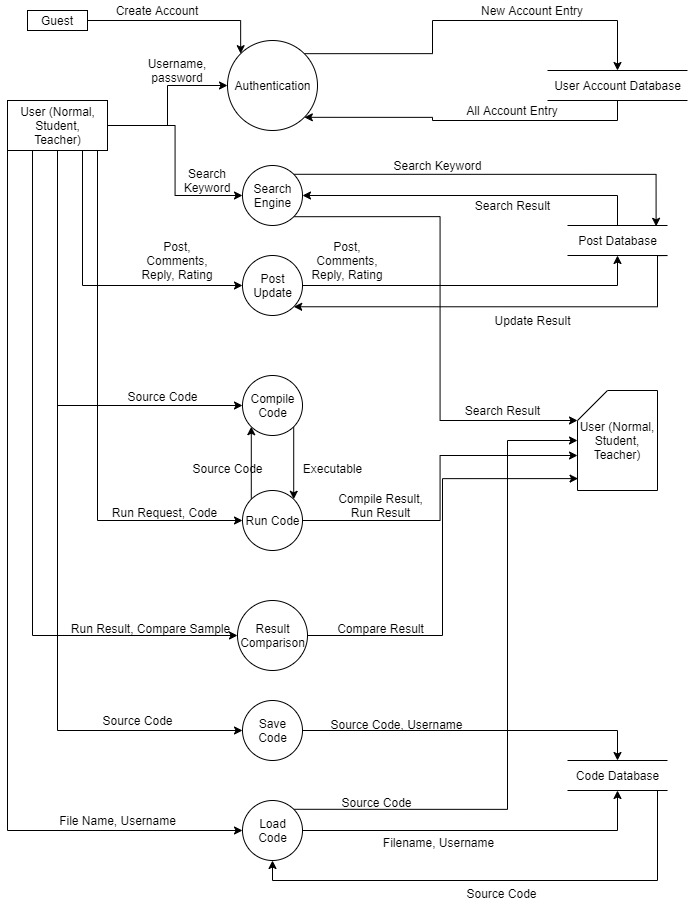
\includegraphics[scale=0.5]{Doc/Graphics/DFD}
